\newcommand{\QtwoCost}{13,832,796.87}
\newcommand{\QtwoCostWan}{1383.2797}
\newcommand{\QtwoPlanCost}{13,487,877.14}
\newcommand{\QtwoEmergencyCost}{344,919.73}
\newcommand{\QtwoSaving}{31,750.39}
\newcommand{\QtwoSaveRate}{0.2290}
\newcommand{\QtwoDaySaving}{10,692.67}
\newcommand{\QtwoCharge}{6,449,842.80}
\newcommand{\QtwoDischarge}{5,224,344.54}
\newcommand{\QtwoUnused}{2,897,584.98}
\newcommand{\QtwoEnd}{6,031.25}

\section{问题二：基于边际价值DP的日前购电与储能控制}
\label{sec:q2}

\subsection{问题分析}

问题二在零点按历史数据制定购电计划，供电不足时按5倍电价补购。多购可能浪费，少购可能增加紧急费用；当前放电还会减少后续可用电量。模型需同时确定用电安全余量和各时段储能用量。

本文先预测负载和光伏，用LP确定当天144个区间的普通购电量，再用边际价值DP决定充放电。全天采用零点确定的普通购电量，剩余缺口由紧急购电补足，储电量逐日延续。

已有储能控制研究表明，在价格波动和效率损耗条件下，动态规划策略常具有阈值结构，并可用有限预测视野刻画库存的边际价值\upcite{vandeven2013storage,cruise2014storage}。结合上述阈值控制思想与本题紧急购电规则，构造储能费用函数。

图\ref{fig:q2-workflow}依次给出历史数据处理、日前购电规划、边际价值DP和结果核验步骤。

\begin{figure}[H]
    \centering
    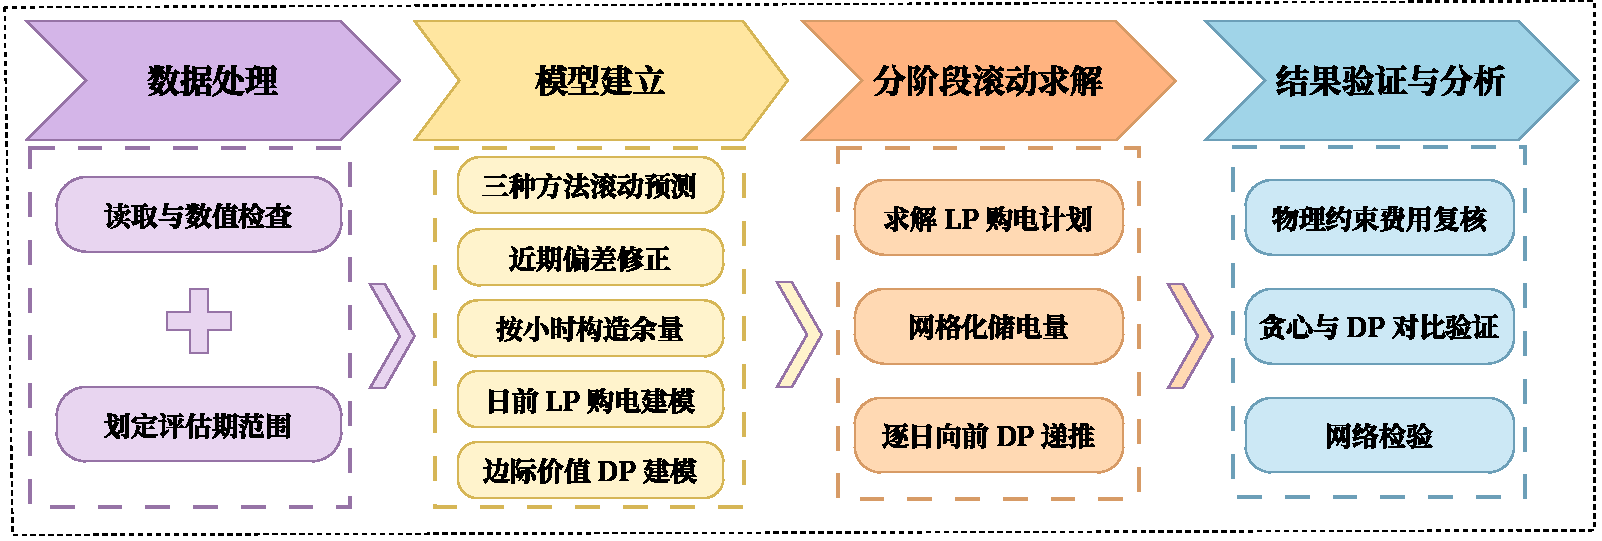
\includegraphics[width=\textwidth]{figures/q2/flowchart2.pdf}
    \caption{问题二流程图}
    \label{fig:q2-workflow}
\end{figure}

\subsection{数据处理}

\textbf{Step 1：整理数据。}附件2含2025年365天、每日144个区间，共52,560组观测。按日期和区间匹配，沿用问题一的电量换算并检查完整性及数值。1月积累历史误差，储电量保持6000\,kWh；2月1日至12月31日用于评估，共334天、48,096个区间。

\textbf{Step 2：确定可用数据。}第$k$日零点仅使用第$k-1$日及此前观测，$t=0,\ldots,143$。$L_{kt},V_{kt}$为实际负载、光伏电量，$p_t$取附件1电价。日内供需仅用于假设4中的即时控制。

\subsection{模型建立}

\subsubsection{负载、光伏预测与用电安全余量}

\textbf{（1）预测方法的选择。}对负载和光伏分别建立昨日同刻、上周同刻与岭回归（Ridge）三种候选方法。Ridge采用昨日同刻值、上周同刻值、近7日同刻均值、昨日全天均值、日内一二阶正余弦项及周末标记共9个特征；在此前最多60个完整日上标准化特征，以
\begin{equation}
    \min_{a,\boldsymbol\beta}
    \sum_{(j,t)\in\mathcal T_k}
    \bigl(y_{jt}-a-\boldsymbol x_{jt}^{\mathsf T}\boldsymbol\beta\bigr)^2
    +10\|\boldsymbol\beta\|_2^2
    \label{eq:q2-ridge}
\end{equation}
拟合各目标。$\mathcal T_k$只包含当日之前可用于训练的日期，标准化参数也只从该训练集计算。

三种候选方法均按日向前滚动拟合。在2025年历史数据的同条件比较中，固定Ridge的负载和光伏RMSE均略低于按此前14日误差逐日选择预测方法的对照方案。综合预测误差、费用对照与模型简洁性，主方案采用固定Ridge，并以逐日选取预测方法作对照。

\textbf{（2）偏差修正。}针对近期连续高估或低估，利用最近3个已完成日的基础预测误差均值修正当天预测。对$y\in\{L,V\}$，令
\begin{equation}
    \widehat y_{kt}^{\,\mathrm{cor}}
    =\max\left\{0,\widehat y_{kt}^{\,\mathrm{base}}
      +\frac{1}{|\mathcal B_k|}\sum_{j\in\mathcal B_k}
       (y_{jt}-\widehat y_{jt}^{\,\mathrm{base}})\right\},
    \qquad \widehat N_{kt}=\widehat L_{kt}^{\,\mathrm{cor}}
                           -\widehat V_{kt}^{\,\mathrm{cor}}.
    \label{eq:q2-bias}
\end{equation}
其中$\mathcal B_k$为最近3个完整日期。修正后的光伏与负载预测均限制为非负值，净负载允许为负，以保留光伏富余信息。

\textbf{（3）按小时构造安全余量。}定义历史修正净负载误差
$r_{jt}=L_{jt}-V_{jt}-\widehat N_{jt}$。对当前区间所属小时$h(t)$，汇集过去14天同一小时6个区间的误差，得到经验样本集$\mathcal R_{k,h(t)}$，评估期内每集有84个样本。取
\begin{equation}
    m_{kt}=\max\{0,Q_{0.8}(\mathcal R_{k,h(t)})\},
    \label{eq:q2-margin}
\end{equation}
作为加在预测负载上的安全余量。净负载被低估时，增加这一余量可提前安排更多供电，减少紧急购电，但也可能增加未用完的已购电量。

在单时段无储能模型中，若随机需求为$X$，最小化$pq+5p\,\mathbb E[(X-q)^+]$的一阶条件为$F_X(q)=0.8$。据此取历史误差的80\%分位数作为用电安全余量。

\subsubsection{日前计划购电模型}

记$\bar c_{kt},\bar d_{kt},\bar E_{kt},\bar w_{kt}$为计划充电量、放电量、储电量和未利用电量，$q_{kt}$为零点确定的购电量。将修正后的预测和安全余量代入，得到
\begin{equation}
\begin{aligned}
    \min\quad &\sum_{t=0}^{T-1}p_tq_{kt},\\
    \text{s.t.}\quad
    &q_{kt}+\widehat V_{kt}^{\,\mathrm{cor}}+\bar d_{kt}
      =\widehat L_{kt}^{\,\mathrm{cor}}+m_{kt}+\bar c_{kt}+\bar w_{kt},\\
    &\bar E_{k,t+1}=\bar E_{kt}+\eta_c\bar c_{kt}-\bar d_{kt}/\eta_d,\\
    &E_{\min}\leq\bar E_{kt}\leq E_{\max},\quad
      0\leq\bar c_{kt},\bar d_{kt}\leq P_{\max}\Delta t,\\
    &q_{kt},\bar w_{kt}\geq0,\qquad
      \bar E_{k0}=E_{k0},\quad\bar E_{kT}=6000.
\end{aligned}
\label{eq:q2-dayahead}
\end{equation}
效率、功率与容量参数沿用问题一。求解LP后，若同一时段同时充放电，则扣除两者相互抵消的部分，保持相同的储电量变化，并检查运行约束。

普通购电价格$p_t$低于紧急价格$5p_t$，普通购电量取非负值，可覆盖全部预测需求，因此日前计划采用普通购电。式\eqref{eq:q2-dayahead}只确定$q_{kt}$；实际充放电随供需调整。

\subsubsection{边际价值DP模型}

普通购电费$\sum_t p_tq_{kt}$已固定，执行时只需权衡当前紧急费用与保留电量的后续价值。$\mathcal V_{k,t}(E)$表示时段$t$开始、储电量为$E$时，按经验误差分布估计的剩余紧急费用与日末补电费用估计。

\textbf{（1）充放电量与供电缺口。}对于误差样本$r\in\mathcal R_{k,h(t)}$，令
\begin{equation}
    x_{kt}(r)=q_{kt}-(\widehat N_{kt}+r).
    \label{eq:q2-balance-sample}
\end{equation}
当$x_{kt}(r)\geq0$时，供电有剩余。模型允许弃用余电，额外储电费用和电池老化费用均设为0，因此在功率与容量允许时尽量充电：
\begin{equation}
    c=\min\left\{x_{kt}(r),P_{\max}\Delta t,
       \frac{E_{\max}-E}{\eta_c}\right\},\quad
    d=u=0,\quad E'=E+\eta_c c.
    \label{eq:q2-charge}
\end{equation}
当$x_{kt}(r)<0$时，缺口为$g=-x_{kt}(r)$，动作满足
\begin{equation}
    0\leq d\leq\min\{g,P_{\max}\Delta t,\eta_d(E-E_{\min})\},
    \qquad u=g-d,\quad c=0,\quad E'=E-d/\eta_d.
    \label{eq:q2-discharge}
\end{equation}
上述动作均满足充放电互斥约束，且紧急购电仅用于补足负载缺口。

\textbf{（2）Bellman递推。}以$\mathcal A(E,r)$表示上述可行动作集，有
\begin{equation}
    \mathcal V_{k,t}(E)
    =\frac{1}{84}\sum_{r\in\mathcal R_{k,h(t)}}
       \min_{a\in\mathcal A(E,r)}
       \left\{5p_tu(a,r)+\mathcal V_{k,t+1}(E'(a,r))\right\}.
    \label{eq:q2-bellman}
\end{equation}
控制器按当前供需选择动作，后续费用按历史误差样本取平均。安全余量$m_{kt}$通过日前计划$q_{kt}$计入，式\eqref{eq:q2-balance-sample}采用预测净负载与误差样本。每个小时的84个残差样本按相同权重组成历史残差分布，递推时按当前小时的分布独立计算各时段误差，状态变量只保留储电量。近3日偏差修正用于处理连续高估或低估。

\textbf{（3）日末补电费用估计。}除评估期最后一天外，以补足日末参考储电量所需的费用估计电量对次日的价值：
\begin{equation}
    \mathcal V_{k,T}(E)=\kappa_k(6000-E)^+,
    \qquad
    \kappa_k=\begin{cases}
    \min_t p_t/\eta_c=0.4125556,&k\text{非12月31日},\\
    0,&k\text{为12月31日}.
    \end{cases}
    \label{eq:q2-terminal}
\end{equation}
其中$(a)^+=\max(a,0)$。该费用按附件1电价估算，用于确定当日留电量。实际储电量连续传至次日。

\subsubsection{放电量的确定}

发生缺口$g$时，令下一时刻储电量为$e$，则$d=\eta_d(E-e)$。去掉费用中与动作无关的项，求得建议保留的储电量

\begin{equation}
    e_{kt}^{\star}\in\arg\min_e
      \{\mathcal V_{k,t+1}(e)+5p_t\eta_de\},
    \label{eq:q2-threshold}
\end{equation}
结合当前储电量、供电缺口和放电功率限制，确定下一时刻储电量：
\begin{equation}
\begin{aligned}
    e_{\mathrm{lo}}&=\max\{E_{\min},E-\min(g,P_{\max}\Delta t)/\eta_d\},\\
    E'&=\min\{E,\max(e_{\mathrm{lo}},e_{kt}^{\star})\},\qquad
    d=\eta_d(E-E'),\quad u=g-d.
\end{aligned}
\label{eq:q2-projection}
\end{equation}
若多个储电量对应的费用相同，选择较小的下一时刻储电量，即优先多放电；未来价值为零时，该规则与贪心放电一致。

内部每放出1\,kWh，可供电$\eta_d$\,kWh，节省当前紧急费用$5p_t\eta_d$元；保留该电量的边际价值可表示为$-\partial_E\mathcal V_{k,t+1}(E)$。前者较大时放电，后者较大时留电；后一情形可能在仍有可放电库存时发生紧急购电。

\subsection{模型求解}

每天确定购电计划后，将$[1200,10800]$按50\,kWh划分为193个储电量点，计算145个时刻对应的预计费用。按84个误差样本，从日末向前计算建议保留电量，网格点之间采用线性插值；主要计算量随$T\times193\times84$增长。

实际储电量保持连续，有富余时按式\eqref{eq:q2-charge}充电，有缺口时按式\eqref{eq:q2-projection}放电并补购。日末储电量传至次日，评估期费用为

\begin{equation}
    J_{\mathrm{year}}=
    \sum_{k=\text{2月1日}}^{\text{12月31日}}
    \sum_{t=0}^{143}(p_tq_{kt}+5p_tu_{kt}).
    \label{eq:q2-annual-cost}
\end{equation}
实际费用由普通购电费和紧急购电费组成，按原始精度累计，年末剩余电量的结算价值设为0。完整结果见\texttt{result2.xlsx}。

\subsection{求解结果}

\subsubsection{全年费用与运行概况}

334天内，普通计划购电量为22,000,180.73\,kWh，计划费为\QtwoPlanCost 元，紧急购电量为62,092.01\,kWh。

交流侧累计充电\QtwoCharge\,kWh、放电\QtwoDischarge\,kWh。

年末储电量为\QtwoEnd\,kWh。紧急购电覆盖125天、743个十分钟区间，按同日连续区间合并为267次事件。

\subsubsection{指定日期购电、储能与紧急结果}

表\ref{tab:q2-purchase}汇总3月20日、6月21日、9月23日、12月21日六个指定区间及全天购电结果，时间均按题面实际区间标注。

\begin{table}[H]
    \centering\small
    \caption{指定日期计划购电量及全天费用（区间电量单位：kWh）}
    \label{tab:q2-purchase}
    \renewcommand{\arraystretch}{1.15}
    \begin{tabularx}{\textwidth}{@{}>{\columncolor{white}[0pt][\tabcolsep]}lRRR>{\columncolor{white}[\tabcolsep][0pt]}R@{}}
\toprule
\rowcolor{paperpale}
时间段 & \mbox{3月20日} & \mbox{6月21日} & \mbox{9月23日} & \mbox{12月21日} \\
\midrule
10:00--10:10 & 0.00 & 0.00 & 0.00 & 0.00 \\
\rowcolor{paperstripe} 12:00--12:10 & 577.64 & 0.00 & 566.93 & 891.93 \\
14:00--14:10 & 0.00 & 0.00 & 0.00 & 0.00 \\
\rowcolor{paperstripe} 16:00--16:10 & 458.29 & 184.77 & 590.06 & 803.03 \\
18:00--18:10 & 719.95 & 0.00 & 802.73 & 706.46 \\
\rowcolor{paperstripe} 20:00--20:10 & 0.00 & 0.00 & 0.00 & 0.00 \\
全天计划量/kWh & 69,398.18 & 35,846.18 & 73,127.12 & 95,682.81 \\
\rowcolor{paperstripe} 全天总费用/元 & 42,373.78 & 20,535.18 & 45,859.13 & 61,758.73 \\
\bottomrule
\end{tabularx}


\end{table}

表\ref{tab:q2-storage}按6个四小时时段汇总充放电量。段内可先后充放电，各十分钟区间仍满足互斥；每日初始储电量沿用前一日末值。

\begin{table}[H]
    \centering\small
    \caption{指定日期四小时充放电量及日初末储量（单位：kWh）}
    \label{tab:q2-storage}
    \renewcommand{\arraystretch}{1.16}
    \begingroup
\setlength{\tabcolsep}{2pt}
\begin{tabularx}{\textwidth}{@{}>{\columncolor{white}[0pt][\tabcolsep]}lX *{3}{rrX}r>{\columncolor{white}[\tabcolsep][0pt]}r@{}}
\toprule
\rowcolor{paperpale} 时间段 &  & \multicolumn{2}{c}{\mbox{3月20日}} &  & \multicolumn{2}{c}{\mbox{6月21日}} &  & \multicolumn{2}{c}{\mbox{9月23日}} &  & \multicolumn{2}{>{\columncolor{white}[\tabcolsep][0pt]}c@{}}{\mbox{12月21日}} \\
\rowcolor{paperpale} &  & 充电 & 放电 &  & 充电 & 放电 &  & 充电 & 放电 &  & 充电 & 放电  \\
\midrule
00:00--04:00 &  & 4,168.47 & 122.38 &  & 826.81 & 864.24 &  & 4,447.45 & 17.16 &  & 3,909.86 & 229.70  \\
\rowcolor{paperstripe} 04:00--08:00 &  & 833.85 & 4,466.23 &  & 540.97 & 4,391.89 &  & 259.29 & 5,668.57 &  & 1,516.35 & 1,687.53  \\
08:00--12:00 &  & 6,252.33 & 2,777.38 &  & 8,951.05 & 0.00 &  & 6,243.34 & 1,896.62 &  & 5,324.81 & 7,297.48  \\
\rowcolor{paperstripe} 12:00--16:00 &  & 2,747.15 & 493.27 &  & 0.00 & 0.00 &  & 3,331.19 & 577.97 &  & 7,637.69 & 2,395.37  \\
16:00--20:00 &  & 391.13 & 5,648.45 &  & 172.05 & 5,646.82 &  & 242.68 & 5,465.73 &  & 54.12 & 5,559.56  \\
\rowcolor{paperstripe} 20:00--24:00 &  & 5,754.18 & 2,986.10 &  & 6,271.88 & 2,499.72 &  & 6,082.83 & 2,778.09 &  & 5,887.87 & 2,842.53  \\
0:00储电量 &  & \multicolumn{2}{r}{6,684.66} &  & \multicolumn{2}{r}{7,353.19} &  & \multicolumn{2}{r}{6,816.36} &  & \multicolumn{2}{>{\columncolor{white}[\tabcolsep][0pt]}r@{}}{7,120.74} \\
\rowcolor{paperstripe} 24:00储电量 &  & \multicolumn{2}{r}{6,490.60} &  & \multicolumn{2}{r}{7,547.81} &  & \multicolumn{2}{r}{7,135.64} &  & \multicolumn{2}{>{\columncolor{white}[\tabcolsep][0pt]}r@{}}{6,782.63} \\
\bottomrule
\end{tabularx}


\endgroup

\end{table}

\begin{table}[H]
    \centering\small
    \caption{指定日期紧急购电结果}
    \label{tab:q2-emergency}
    \renewcommand{\arraystretch}{1.15}
    \begin{tabularx}{\textwidth}{@{}>{\columncolor{white}[0pt][\tabcolsep]}lRRR>{\columncolor{white}[\tabcolsep][0pt]}R@{}}
\toprule
\rowcolor{paperpale} 指标 & \mbox{3月20日} & \mbox{6月21日} & \mbox{9月23日} & \mbox{12月21日} \\
\midrule
紧急购电时间段 & 无 & 无 & 无 & 07:50--08:00 \\
\rowcolor{paperstripe} 紧急电量/kWh & 0.00 & 0.00 & 0.00 & 14.55 \\
\bottomrule
\end{tabularx}


\end{table}

表\ref{tab:q2-emergency}显示，12月21日07:50--08:00发生14.55\,kWh紧急购电，其余三个指定日期的紧急购电量在$10^{-7}$\,kWh容差内记为0。全年事件按“十分钟区间数、同日连续事件数、发生天数”分别统计，详见工作簿。

\subsubsection{储能控制实例}

以节费较大的2025年9月8日为例，图\ref{fig:q2-mechanism}比较相同计划下贪心与DP的储电量和紧急购电。

\begin{figure}[H]
    \centering
    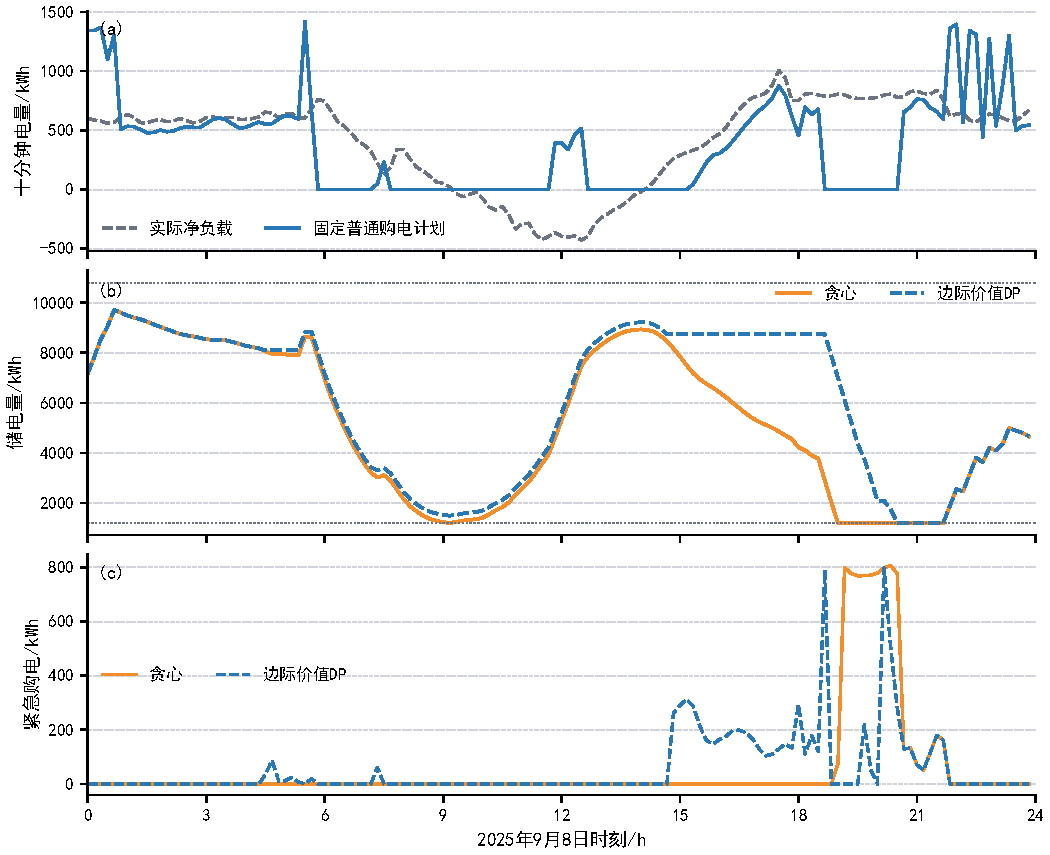
\includegraphics[width=\textwidth]{figures/q2/q2_dp_mechanism.pdf}
    \caption{9月8日相同购电计划下两种储能控制方法的运行轨迹}
    \label{fig:q2-mechanism}
\end{figure}

04:40--04:50的供电缺口为90.40\,kWh，电价为0.4422元/kWh。贪心控制立即放电；DP建议保留8150\,kWh，高于当时的8105.12\,kWh储电量，因此支付199.88元紧急购电费并将电量留至后续高价时段。该日DP节省\QtwoDaySaving 元；全年共有295个区间在能够放电时选择留电并紧急购电。

\subsection{模型检验}

下述费用差区间均以两种方法的配对逐日费用差为样本，采用7日连续块重采样，重复10000次，随机种子取2026。

\subsubsection{预测检验}

按各日零点可用信息计算48,096个区间的误差。固定Ridge的负载、光伏RMSE分别为39.44、56.99\,kWh，逐日选取预测方法分别为39.87、57.06\,kWh。将两种方法的年末储电量统一为6000\,kWh后，逐日选取预测方法比固定Ridge多支出0.5912万元，95\%重采样区间为$[-2.1451,3.0413]$万元，区间跨越零点。表\ref{tab:q2-forecast-selection}给出同条件比较；固定Ridge的紧急区间略多，但补购时点的费用更低。

\begin{table}[H]
    \centering\small
    \caption{统一6000 kWh年末储电量下固定Ridge与逐日选取预测方法的比较}
    \label{tab:q2-forecast-selection}
    \renewcommand{\arraystretch}{1.15}
    \begin{tabularx}{\textwidth}{@{}>{\columncolor{white}[0pt][\tabcolsep]}lRRRR>{\columncolor{white}[\tabcolsep][0pt]}R@{}}
\toprule
\rowcolor{paperpale} 预测方案 & 负载RMSE & 光伏RMSE & 总费用/万元 & 紧急电量/kWh & 紧急区间数 \\
\midrule
逐日选取预测方法 & 39.87 & 57.06 & 1384.3210 & 60574.70 & 704 \\
\rowcolor{paperstripe} 固定Ridge & 39.44 & 56.99 & 1383.7298 & 62092.01 & 743 \\
\bottomrule
\end{tabularx}

\end{table}

\subsubsection{相同购电计划下的储能控制比较}

固定普通购电计划、实际供需、电价、初始储电量及物理参数，仅将DP换为“有缺口就尽量放电”的贪心控制，连续运行334天（表\ref{tab:q2-comparison}）。两者使用同一份冻结购电计划，计划费和年末储电量相同。

\begin{table}[H]
    \centering\small
    \caption{冻结同一普通购电计划后的储能控制方法费用比较}
    \label{tab:q2-comparison}
    \renewcommand{\arraystretch}{1.15}
    \begin{tabularx}{\textwidth}{@{}>{\columncolor{white}[0pt][\tabcolsep]}lRRR>{\columncolor{white}[\tabcolsep][0pt]}R@{}}
\toprule
\rowcolor{paperpale} 储能控制方法 & 计划费用/万元 & 紧急费用/万元 & 总费用/万元 & 年末储电量/kWh \\
\midrule
贪心反馈 & 1348.7895 & 37.6670 & 1386.4565 & 6,031.25 \\
\rowcolor{paperstripe} 边际价值DP & 1348.7895 & 34.4920 & 1383.2815 & 6,031.25 \\
\bottomrule
\end{tabularx}

\end{table}

表\ref{tab:q2-comparison}中的DP沿用冻结购电计划，总费用为1383.2815万元；主方案按每日实际初始储电量重新求解购电计划，总费用为1383.2797万元，两者相差18.12元。贪心与DP的紧急电量分别为61,931.41\,kWh和62,092.01\,kWh。DP通过转移补购时点，在冻结计划下节省3.1750万元；每日重新规划并统一年末储电量后节省3.1769万元，95\%重采样区间为$[1.1640,6.1129]$万元。

\subsubsection{数据时序检验}

将附件4电价整体替换为极端常数后重新运行，购电计划、储能动作和总费用保持不变，两次运行得到的完整结果文件完全一致。因此，本问的预测、规划与执行仅依赖附件1--2以及决策时已经发生的历史信息。



\subsubsection{网格检验}

在同一固定普通购电计划下，将储电网格改为100、25\,kWh，结果见表\ref{tab:q2-grid}。三档网格的最大费用差为358.65元，占总费用的$0.0026\%$。网格用于近似期望价值函数，年度费用由实际运行轨迹计算。50\,kWh在精度与计算量之间较为均衡，故用于主结果。

\begin{table}[H]
    \centering\small
    \caption{固定Ridge与冻结购电计划下的DP网格检验}
    \label{tab:q2-grid}
    \renewcommand{\arraystretch}{1.15}
    \begin{tabularx}{\PaperTableCompactWidth}{@{}>{\columncolor{white}[0pt][\tabcolsep]}rRR>{\columncolor{white}[\tabcolsep][0pt]}R@{}}
\toprule
\rowcolor{paperpale} 网格间距/kWh & 状态点数 & 总费用/万元 & 相对50 kWh费用差/元 \\
\midrule
100.00 & 97 & 1383.3119 & +304.22 \\
\rowcolor{paperstripe} 50.00 & 193 & 1383.2815 & 0.00 \\
25.00 & 385 & 1383.2761 & $-54.43$ \\
\bottomrule
\end{tabularx}


\end{table}

\subsection{结论}

评估期主方案总费用为\QtwoCostWan{}万元，其中计划购电费1348.7877万元、紧急购电费34.4920万元。在冻结同一普通购电计划并统一两种控制方法的初始、年末储电量后，DP较贪心节省3.1750万元，降幅为\QtwoSaveRate\%。
